\subsection{Eigenvalue Estimators}\label{ss:eigenvalue}

One of the most important results of interest for this problem is how k-eff changes as the pin pitch is modified.  This result is shown on the next page in Fig. \ref{f:keffVpitch}.  Out of the simulations that were run, the maximum k-effs are 1.07066 $\pm$ 0.00036 (track-length) and 1.07174 $\pm$ 0.00030 (collision), which both occur at a pin pitch of 4.5 cm.

The shape of the curve is due to the fuel-to-moderator ratio.  At the smallest pin pitches, there is little moderator to slow down the neutrons, so they usually just get absorbed in the fuel instead of thermalizing and causing fission.  This effect would be mitigated some if fast fission in U-238 were considered in this model, but it is not.  For the largest pitches, there is a greater chance of neutrons being absorbed in the moderator, or simply never returning to the fuel after thermalizing.  Beginning at a pitch of 4.75 cm, this effect begins to dominate the benefits of moderation.

The reported uncertainty on the track-length estimator ranged from 31.4 pcm to 36.7 pcm.  For the collision estimator, they ranged from 27.2 pcm to 30.5 pcm. In this case, it appears that both estimators are approximately equivalent. If surface crossings were more prevalent (e.g. if axial or radial divisions were included), then the track-length estimator would be much more effective than the collision estimator. However, because there are only two distinct spatial regions in the problem (fuel and moderator), the collision estimator works very well. There is actually less variance with the collision estimator because the natural variance in track lengths is incorporated into the track-length estimator. For most cases, the difference between the track-length and collision estimates of keff is less than 100 pcm. This is not surprising, considering that the estimated 1-$\sigma$ uncertainty in the estimators is about 30 pcm each, and we know that this is an underestimate due to correlation between cycles.

\subsection{Leakage Estimators}\label{ss:leakage}

A second quantity of interest is the leakage out of the pin cell, which is shown in Fig. \ref{f:leakVpitch}.  The leakage curves have some fluctuation in them, but generally have the same shape and similar magnitudes.  This is to be expected, since the problem is axially symmetric.  It also decreases with increasing pin pitch.  This occurs because the increase in the amount of moderator slows down the neutrons more effectively, which decreases their mean free path and reduces the probability of escaping the pin cell.

For both figures, error bars are included, but too small to be easily visible.  For Fig. \ref{f:keffVpitch}, this might be acceptable, but for Fig. \ref{f:leakVpitch} we would expect to see the two curves lying within each other's uncertainties.  However, in lecture it stated that the uncertainties which are reported are usually much lower than they should be.  This is due to the fact that all the neutrons in the active cycles are correlated to their predecessors, but uncertainty calculations assume completely independent samples.  Thus, this correlation makes the distributions appear more exact than they are.  This, combined with how relatively few scores occur on each of these estimators, explains why there is some discrepancy between the top and bottom leakages.

\begin{figure}[H]
\centering
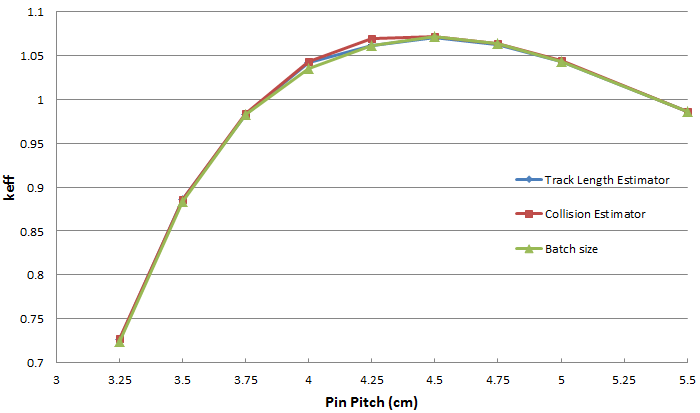
\includegraphics[width=0.8\linewidth]{images/keff.png}
\caption{Plot of track-length (blue) ,  collision (red) , and batch size (green) estimators of k-eff versus pin pitch}
\label{f:keffVpitch}
\end{figure}

\begin{figure}[H]
\centering
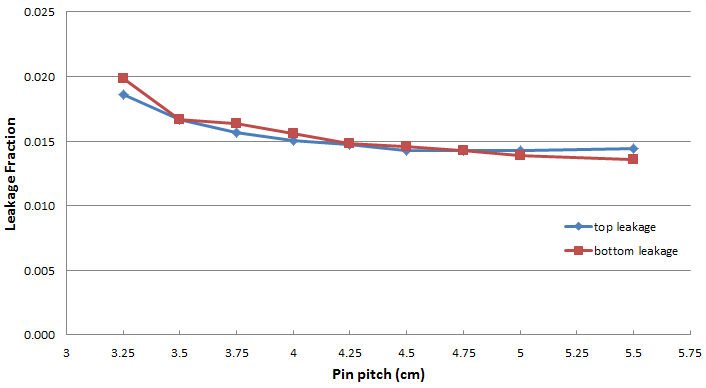
\includegraphics[width=0.8\linewidth]{images/leakage.png}
\caption{Plot of top (blue) and bottom (red) leakages versus pin pitch}
\label{f:leakVpitch}
\end{figure}

\subsection{Fission Source Convergence}\label{ss:fissionconv}

The Shannon Entropy of the fission source was used to determine convergence. As shown in Fig. \ref{f:entropy}, the entropy decreases as the source converges from the initial flat guess to the dominant eigenfunction. The Shannon entropy converges close to a mean value after about 15-20 iterations, so we chose to use 20 inactive cycles. Each run used $10^5$ particles per batch, with 200 total cycles (20 inactive and 180 active). The mesh used to calculate the entropy had 10 radial divisions and 100 axial divisions. Azimuthal divisions were not used because the problem is nearly (not quite) symmetric azimuthally. The source should vary weakly azimuthally compared to the variation in the radial and axial directions within the pin.

\begin{figure}[H]
\centering
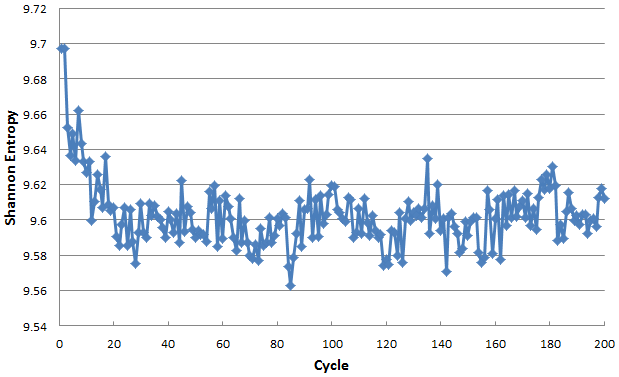
\includegraphics[width=0.8\linewidth]{images/Entropy.png}
\caption{Convergence of Shannon Entropy to a mean value}
\label{f:entropy}
\end{figure}

\subsection{Energy Spectrum}\label{ss:spectrum}

While this problem used a relatively simple functional form for the cross sections instead of a large table of hyperfine/continuous energy cross sections, the energy spectrum is still of great interest.  In the figures below, we can see the two large peaks at either end of the spectrum: the peak in the fast flux from the Watt spectrum, and the peak in the thermal flux from neutrons reaching thermal equilibrium. In the slowing down range, where the flux would be flat without absorption, we can see a slope due to absorption during slowing-down. The 3 resonances that were defined for U-238 can be seen clearly in the fuel spectrum, and if the pitch is small enough, the dip also appears in the moderator spectrum (although less pronounced). 

The energy range from 3 meV to 30 MeV was divided into logarithmically-spaced bins, and the flux in both the fuel and moderator regions was tallied using 200 cycles and $10^4$ neutrons per cycle. The pitch was varied between 3.5 cm and 5.0 cm to demonstrate the effect of fuel-to-moderator ratio on the energy spectrum.

With the pitch at 4 cm, the fast flux is much higher than the thermal flux because there is not enough moderation \ref{f:spectrumlowmod}. Because we are not modeling fast fission in this problem, there will be a reactivity penalty for a lack of moderation (namely, more absorption in the fuel before reaching thermal energy). For the 5 cm pitch (Fig. \ref{f:spectrumhighmod}), there is plenty of moderation: the relative size of the thermal flux peak to the fast flux peak in the fuel is increased from approximately 1:5 at 4 cm to about 1:3 at 5 cm. However, the moderator spectrum goes from a 1:2 thermal to fast flux peak to a slightly higher thermal flux peak. Because absorption in the moderator is stronger at thermal energies, the absorption in the moderator is much higher at a pitch of 5 cm. At the same time, the slope of the spectrum in the slowing down range is shallower with the larger pitch, indicating less absorption in the slowing-down energy range. This makes sense because there is effectively more moderator between each fuel pin in the infinite lattice, so the fuel will see fewer of these neutrons and fast/epithermal absorption will be lower. 

The peak in keff occurred at a pitch of 4.5 cm (Fig. \ref{f:spectrummedhighmod}, where there is a good balance between moderation and thermal absorption in the moderator. With a pitch of 3.5 cm, there is more fuel than moderator, so the thermal flux is very low compared to the fast flux (Fig. \ref{f:spectrumlowmod}), and keff is very low as a result. Also, there is less difference between the fuel spectrum and the moderator spectrum when there is less moderator.

\begin{figure}[H]
\centering
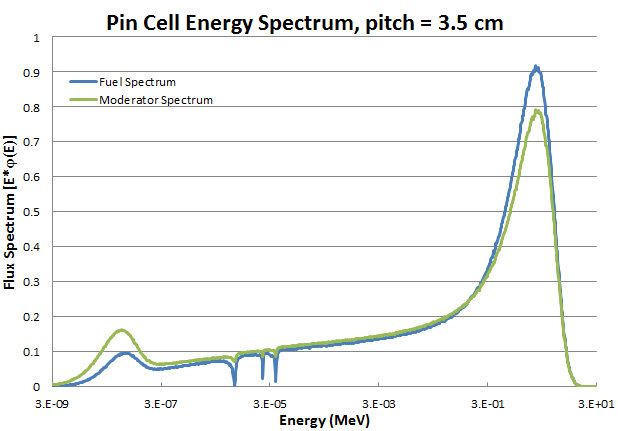
\includegraphics[width=0.8\linewidth]{images/spectrum_lowmod.png}
\caption{Flux Spectrum with pitch = 3.5 cm (low moderation)}
\label{f:spectrumlowmod}
\end{figure}

\begin{figure}[H]
\centering
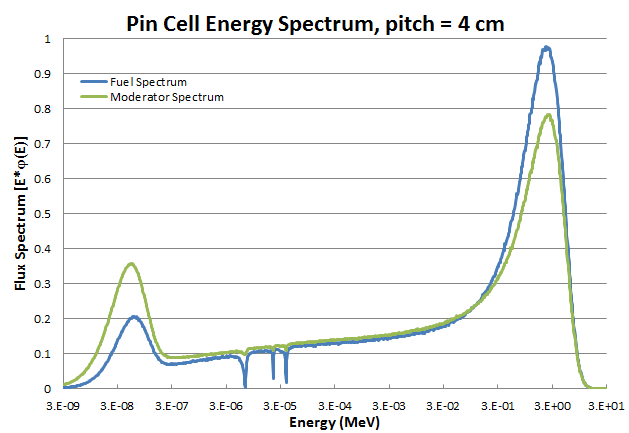
\includegraphics[width=0.8\linewidth]{images/spectrum_medlowmod.png}
\caption{Flux Spectrum with pitch = 4.0 cm (medium low moderation)}
\label{f:spectrummedlowmod}
\end{figure}

\begin{figure}[H]
\centering
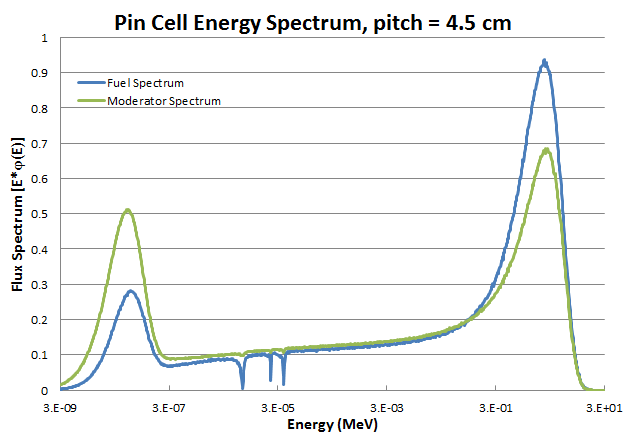
\includegraphics[width=0.8\linewidth]{images/spectrum_medhighmod.png}
\caption{Flux Spectrum with pitch = 4.5 cm (medium high moderation)}
\label{f:spectrummedhighmod}
\end{figure}

\begin{figure}[H]
\centering
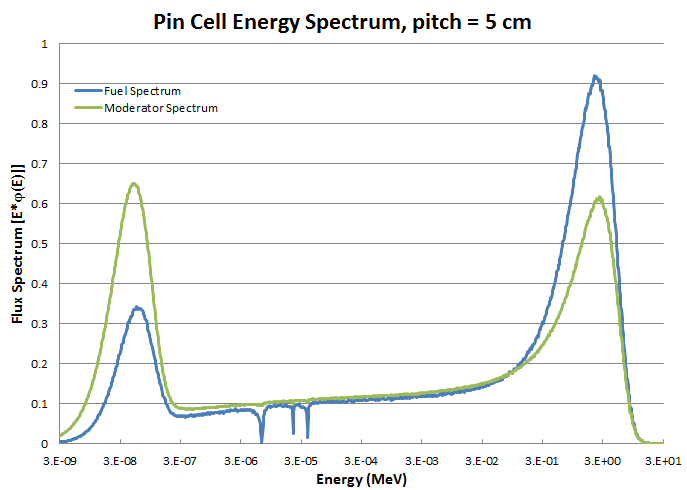
\includegraphics[width=0.8\linewidth]{images/spectrum_highmod.png}
\centering
\caption{Flux Spectrum with pitch = 5.0 cm (high moderation)}
\label{f:spectrumhighmod}
\end{figure}